\subsection{Datapath architecture}
For the implementation of the datapath, the processor described in \autoref{subsection:pipe_arch} was considered as starting point and the architecture shown in \autoref{fig:datapath_architecture} was derived. The five-stage pipelined partition was adopted. In addition, the register file was added in the design but the instruction and data memories were not, as these were only included in the testing phase.

\begin{figure}[h]
  \center
  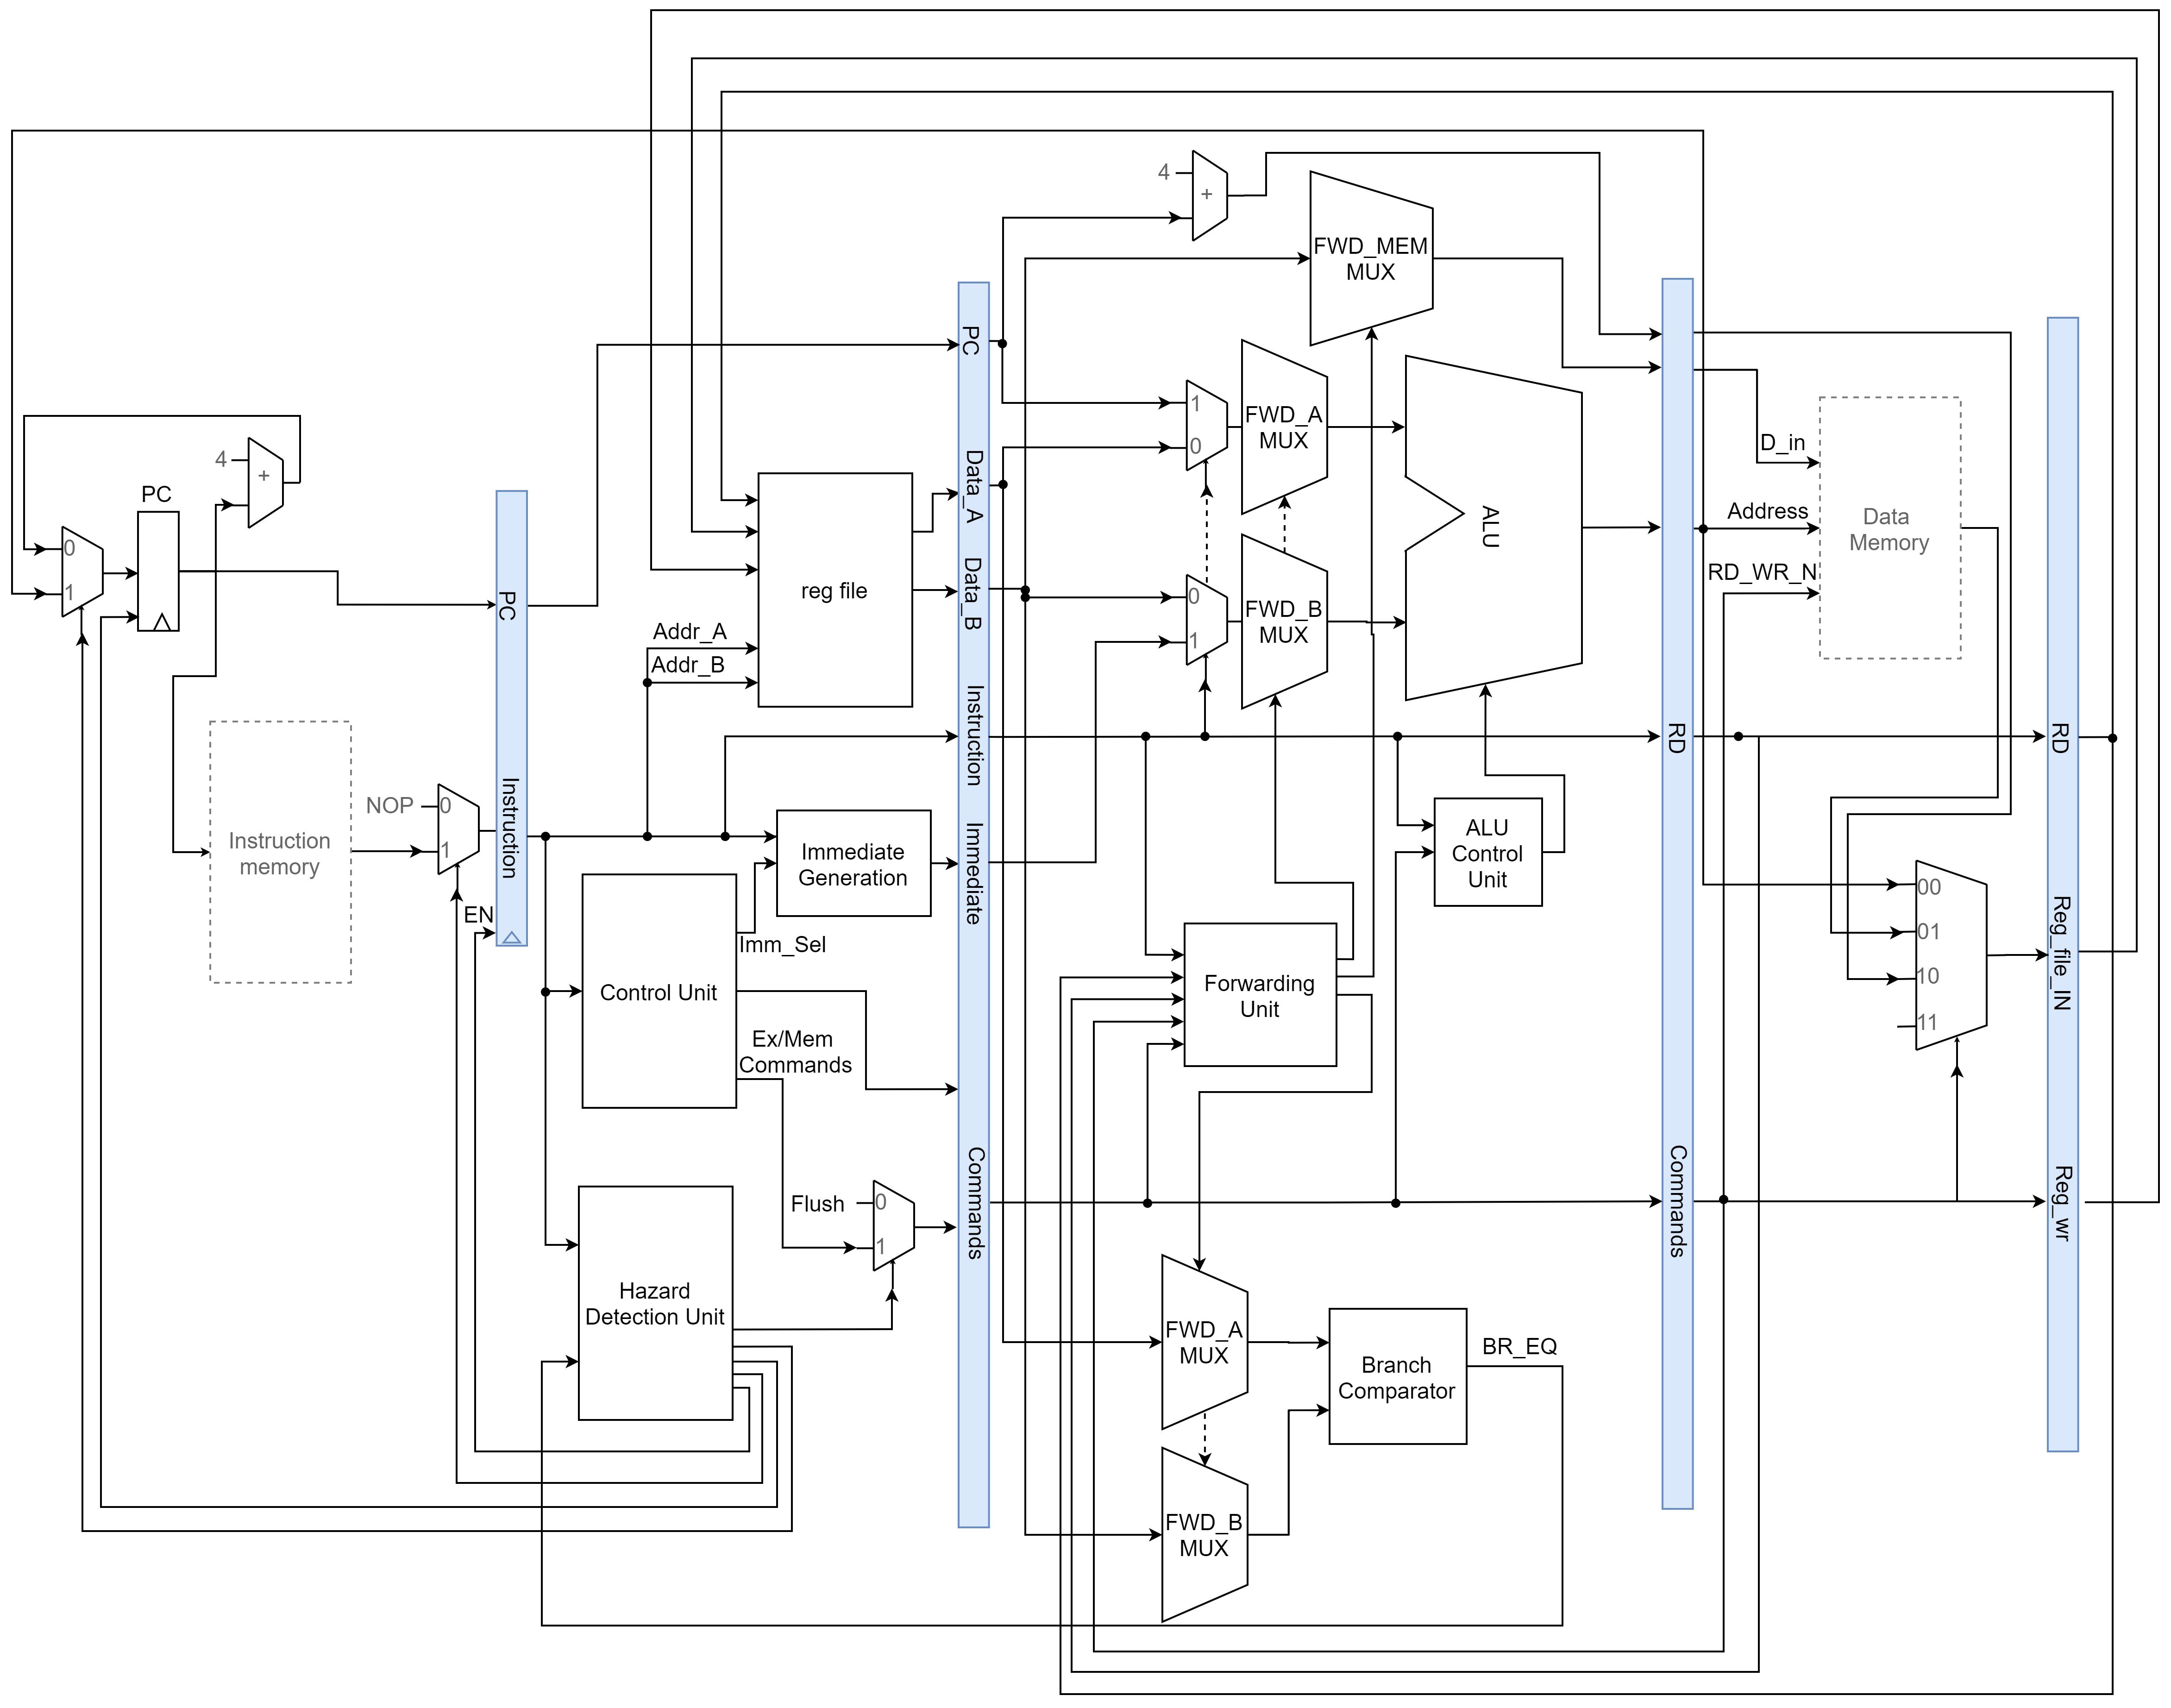
\includegraphics[width=1\textwidth]{sec2/images/datapath.png}
  \caption{Datapath architecture}
  \label{fig:datapath_architecture}
\end{figure}
